\section{Trig (I): Right Triangle and Unit Circle}

\subsection{Review problems}

\begin{enumerate}
\item \emph{Unit conversions for angles.}
\begin{enumerate}
\item 360 degrees to radians
\item $\pi$ radians to degrees
\item 60 degrees to radians
\item $3\pi/4$ radians to degrees
\item $\pi/5$ degrees to radians
\end{enumerate}
\item \emph{Trig functions as ratios of lengths.} Let $ABC$ be a triangle with a right angle at $B$. Suppose $AB = 8$ and $BC = 15$.
\begin{enumerate}
\item Evaluate $\tan A$ and $\cot A$.
\item Find the length of $AC$.
\item Evaluate $\sin A$, $\cos A$, $\sec A$, and $\csc A$.
\end{enumerate}
\item \emph{Using one trig function to compute another.} Throughout, assume $\theta$ is acute.
\begin{enumerate}
\item If $\sin\theta = 1/3$, what is $\cos\theta$?
\item If $\sec\theta = \sqrt{10}$, what is $\tan\theta$?
\item If $\tan\theta = 2/5$, what is $\csc\theta$?
\end{enumerate}
\item \emph{Important acute angles.}
\begin{center}
\begin{tabular}{c|c||c|c|c|c|c|c}
$\theta$ (deg) & $\theta$ (rad) & $\sin\theta$ & $\cos\theta$ & $\tan\theta$ & $\sec\theta$ & $\csc\theta$ & $\cot\theta$ \\ \hline
 & & & & & & & \\
30 & & & & & & & \\
 & & & & & & & \\ \hline
 & & & & & & & \\
45 & & & & & & & \\
 & & & & & & & \\ \hline
 & & & & & & & \\
 & $\pi/3$ & & & & & & \\
 & & & & & & & 
\end{tabular}
\end{center}\newpage
\item \emph{Unit circle calculations.}
\begin{enumerate}
\item $\cos(0)$
\item $\sin(150^{\circ})$
\item $\cos(-3\pi/4)$
\item $\sin(7\pi/3)$
\item $\cos(330^{\circ})$
\item $\sin(-\pi/4)$
\end{enumerate}
\item \emph{Unit circle identities.} Express each of the following in terms of $\sin\theta$ and/or $\cos\theta$.
\begin{enumerate}
\item $\sin(\pi - \theta)$
\item $\cos(\pi - \theta)$
\item $\sin(\pi + \theta)$
\item $\cos(\pi + \theta)$
\item $\sin(-\theta)$
\item $\cos(-\theta)$
\item $\sin(\frac{\pi}{2} - \theta)$
\item $\cos(\frac{\pi}{2} - \theta)$
\item $\sin(\frac{\pi}{2} + \theta)$
\item $\cos(\frac{\pi}{2} + \theta)$
\end{enumerate}
\item \emph{Some triangle geometry.} In acute triangle $ABC$, it is given that $AB = 13$, that $BC = 14$, and that $\sin B = 12/13$.
\begin{enumerate}
\item Find the area of triangle $ABC$.
\item Find the length of $AC$.
\item Find $\sin A$.
\end{enumerate}
\end{enumerate}


\subsection{Challenge problems}

\begin{enumerate}\setcounter{enumi}{7}
\item Much of classical trigonometry was done in terms of the \emph{chord function}, which is defined for angles $0 < \theta < 180^{\circ}$ as follows. Let $O$ be the center of a circle of radius 1, and let $A$ and $B$ be points on the circle so that $\angle AOB = \theta$. Then $\chd\theta$ is defined to be the length $AB$.
\begin{enumerate}
\item Compute $\chd 90^{\circ}$, $\chd 60^{\circ}$, and $\chd 30^{\circ}$.
\item Express $\chd\theta$ in terms of the sine function.
\item Prove that $\chd^2\theta + \chd^2(180^{\circ} - \theta) = 4$.
\end{enumerate}\newpage
\item A method for estimating the distances to the Sun and the Moon using measurements of solar and lunar eclipses dates back to the Greek astronomer Hipparchus (c.\~190 BC to c.\~120 BC). In this problem, we work through the relevant geometric argument.
\begin{figure}[H]
\centering
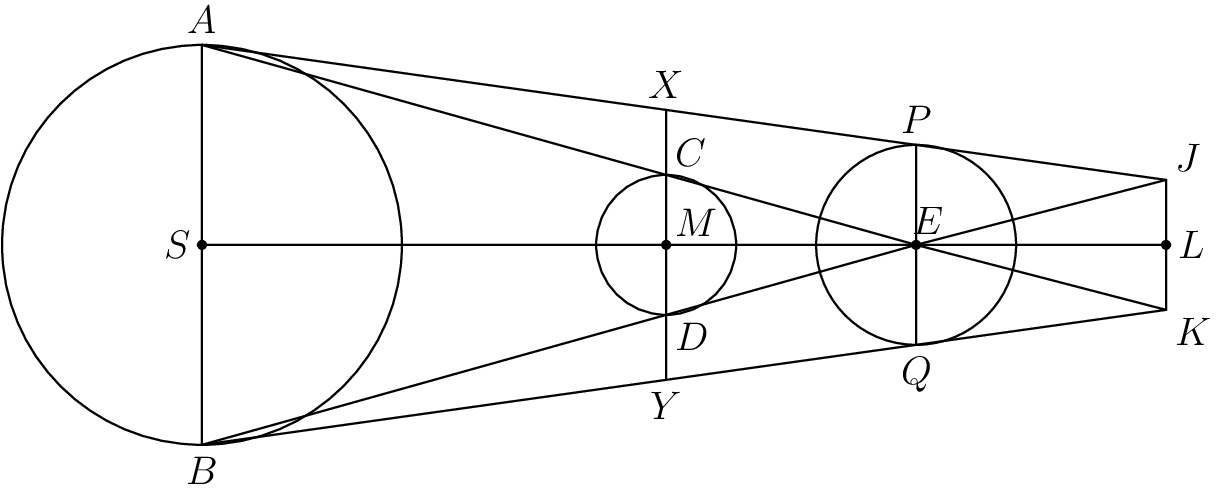
\includegraphics[scale=0.4]{img-hipparchus-2.png}
\end{figure}
In the diagram, points $S$, $M$, $E$, and $L$ lie on a line, with $S$, $M$, and $E$ representing the centers of the Sun, Moon, and Earth, respectively. Segments $\overline{AB}$, $\overline{CD}$, and $\overline{PQ}$ are diameters of their respective circles, all perpendicular to $\overline{SL}$. Segment $\overline{JK}$ is also perpendicular to $\overline{SL}$. Points $A, X, P, J$ are collinear, points $B, Y, Q, K$ are collinear, points $X, C, D, Y$ are collinear, points $A, C, E$ are collinear, and points $B, D, E$ are collinear. Finally, $E$ is the midpoint of $\overline{LM}$. Let $PE = 1$ (so lengths are in terms of Earth radii) and define
\begin{equation*}
\ell = EM = EL,\quad s = ES,\quad\theta = \angle CEM,\quad\phi = \angle JEL.
\end{equation*}
\begin{enumerate}
\item Show that 
\begin{equation*}
s = \frac{\ell}{(\tan\theta + \tan\phi)\ell - 1}
\end{equation*}
\item (Calculator recommended) The measurements used by Hipparchus were
\begin{equation*}
\ell\approx 67\tfrac{1}{3},\quad\theta\approx 0.277^{\circ},\quad\phi\approx 0.693^{\circ}.
\end{equation*}
Given these measurements, what value do we get for $s$?
\item (Calculator recommended) Currently, our measurements for the same quantities are
\begin{equation*}
\ell = 60.268,\quad\theta\approx 0.267^{\circ},\quad\phi\approx 0.746^{\circ}.
\end{equation*}
Given these measurements, what value do we get for $s$?\par
\end{enumerate}
For reference, the true value of $s$ is $s\approx 23{,}455$, so some of the approximations made in order to set up the diagram turn out to be substantial sources of error.\newpage
\item A \emph{Pythagorean triple} is a triple $(X,Y,Z)$ of positive integers for which $X^2 + Y^2 = Z^2$. Note that if $(X,Y,Z)$ is a Pythagorean triple, then $(x,y) = (X/Z, Y/Z)$ is a point on the unit circle whose coordinates are rational numbers.
\begin{enumerate}
\item Let $O = (-1,0)$. If $P\neq O$ has rational coordinates and lies on the unit circle, then the slope of $\overline{OP}$ is rational. Conversely, show that if $\ell$ is a line passing through $O$ which has rational slope, then the other point $P\neq O$ at which $\ell$ intersects the unit circle must have rational coordinates.
\item Use part (a) to show that aside from $O$, every point on the unit circle with rational coordinates can be written in the form $\displaystyle\left(\frac{n^2 - m^2}{n^2 + m^2}, \frac{2mn}{n^2 + m^2}\right)$ for integers $m$ and $n$.
\end{enumerate}
A result going back to Euclid states that every \emph{primitive} Pythagorean triple, meaning a Pythagorean triple $(X,Y,Z)$ where $\gcd(X,Y,Z) = 1$, can be written as either
\begin{equation*}
X = n^2 - m^2,\quad Y = 2mn,\quad Z = n^2 + m^2
\end{equation*}
with $\gcd(m,n) = 1$ and $m + n$ odd, or in the same form with $X$ and $Y$ swapped. The result of part (b) gets most of the way to proving this, with a couple of details to fill in.
\end{enumerate}


%\newpage
%\subsection{Answers}